This chapter is a short introduction to \gls{smc} methods and specifically particle filters. Particle filters were originally developed for object tracking and time series analysis for nonlinear, non-Gaussian state-space models.\cite{Gordon1993}

The term filtering in this context means extracting information about a signal from partial and noisy observations in dynamical systems. In contrast to other estimation problems, filtering is about estimating the current state of a system given only observations up to this point in time.\cite{AppliedOptimalEstimation}

Particle filters are \gls{smc} methods and a subset of \gls{mc} algorithms. They can be used to solve filtering problems arising in signal processing and Bayesian statistical inference. The goal is to compute the posterior distributions of states in a Markov process, given the prior distribution of states and some partial and noisy observations. The term ``particle filter'' was first used by Del Moral in 1996.\cite{Moral1996}

The particle filter uses a set of particles to represent the current state of the system. There is no limitation on the state-space model, the initial state, and the noise distribution of observations.\cite{Moral1996} However, in practice the particle filter does not perform well in very high-dimensional systems. A likelihood is assigned to each particle that represents an approximate probability measure of that particle being sampled from the usually analytically unknown probability density function. A resampling step is necessary to avoid weight disparity leading to weight collapse. There are several adaptive resampling criteria that can be used to avoid bias in that step, including the variance of the weights and the relative entropy with respect to the uniform distribution.\cite{Moral2012} In the resampling step, the particles with negligible weights are replaced by new particles in the proximity of the particles with higher weights.

\section{Filtering with state-space models}

According to Hans Künsch\cite{Kuensch2013}, filtering has been mainly studied in the framework of state-space or hidden Markov models in the last 50 years, assuming a Markovian time evolution of the signal and observations which are instantaneous functions of the signal subject to white observation noise.

The objective of a filter is to estimate the state variables $X_k$ given the observation variables $Y_k$. The observable variables $Y_k$ are related to the hidden variables $X_k$ by some functional form $g(y_k|x_k)$ that is known. Similarly, the dynamics of the state process is also known $f(x_k|x_{k-1})$. A generic state and observation process is illustrated below.

\[\begin{array}{cccccccccc}
X_0 & \to & X_1 & \to & X_2 & \to & X_3 & \to & \cdots & \text{signal} \\
\downarrow & & \downarrow & & \downarrow & & \downarrow & & \cdots & \\
Y_0 & & Y_1 & & Y_2 & & Y_3 & & \cdots & \text{observation}
\end{array}\]

Given the observation process $Y_0,\cdots ,Y_k$ at any time step $k$ sequentially, the filtering problem is to estimate the values of the hidden states $X_k$.

Bayesian estimates of $X_k$ follow from the posterior density $p(x_k|y_0,\cdots,y_k)$. Particle filters provide an approximation of these conditional probabilities by weighted samples. In contrast to \gls{smc} methods, \gls{mcmc} methods would have to deal with the full posterior distribution $p(x_0,\cdots,x_k|y_0,\cdots,y_k)$ for each iteration.

\section{Filtering recursion}

In order to start the recursion, a prior distribution $p(x_0)$ of the hidden state $X_0$ is required. Selecting samples of the prior distribution is called initialization. One has to be careful choosing a prior distribution because it is a potential source of bias. The prior might depend on the first observation $Y_0$ for example.

Given the following observation $Y_0$ we want to update the hidden state of our filter. Following Bayesian's theorem we get the following:

\[p(x_0,x_1|y_1) \sim L(y_1|x_0,x_1)\ p(x_1) = g(y_1|x_1)\ f(x_1|x_0)\ p(x_0)\]

With the likelihood function $L(y_1|x_0,x_1)$ given by the observation function $g(y_k|x_k)$ and $p(x_1)$ by the state evolution function $f(x_k|x_{k-1})$. Following this process recursively and applying normalization yields the following:

\begin{equation}
\label{eq:pf}
    p(x_{1:k}|y_{1:k}) = \frac{g(y_k|x_k)\ f(x_k|x_{k-1})\ p(x_{1:k-1}|y_{1:k-1})}{p(y_k|y_{1:k-1})}\
\end{equation}

With the abbreviation $x_{1:k} = x_1,\cdots,x_k$, the normalization

\[p(y_k|y_{1:k-1}) = \int_{S} g(y_k|x_k)\ f(x_k|x_{k-1})\ p(x_{1:k-1}|y_{1:k-1}) \,dx_k\]

and the state space volume $S$.

By marginalization of \ref{eq:pf} (integration over $x_{1:k-1}$) we derive the following:

\begin{equation}
\label{eq:pf_update}
    p(x_k|y_{1:k}) = \frac{g(y_k|x_k)\ p(x_k|y_{1:k-1})}{p(y_k|y_{1:k-1})}\
\end{equation}

\begin{equation}
\label{eq:pf_prediction}
    p(x_k|y_{1:k-1}) = \int_{V} f(x_k|x_{k-1})\ p(x_{k-1}|y_{1:k-1}) \,dx_{k-1}
\end{equation}

Equation \ref{eq:pf_prediction} is usually called the prediction step and \ref{eq:pf_update} the update step. However, according to Arnaud Doucet\cite{Doucet2011} most particle filtering methods rely on numerical approximations of \ref{eq:pf} instead of \ref{eq:pf_prediction} and \ref{eq:pf_update}.

Analytical solutions are given for two important special cases. The recursion shown above can then be performed exactly. First, when the state space $S$ is finite the integrals above are reduced to finite sums. Second, when the system is linear and $p(x_0)$, $g(y_k|x_k)$, and $f(x_k|x_{k-1})$ are Gaussian the filtering problem can be solved by a Kalman filter exactly.\cite{Kalman1960}

\section{Resampling}

An algorithm that follows the steps initialization, prediction, and update sequentially by representing the distributions with $N$ samples is called \gls{sis}. It can be shown that the variance of the weights is growing exponentially with the number of iterations.\cite{Doucet2011} The important and defining feature of the particle filter is the resampling step which removes particles with low weights and replaces particles with high weights by multiple offspring particles in close proximity. After a resampling step, all particles have the same weight and the distribution is only represented by the number of particles in the different states.

Common algorithms for resampling are \textbf{systematic resampling} and \textbf{multinomial resampling}.\cite{Doucet2011} Both require a summation of all weights which can be a bottleneck for parallelization. Other techniques were discussed by Murray, Lee, and Jacob in 2016.\cite{parallel_resampling}

To avoid unnecessary resampling steps in case of sufficient even weight distribution adaptive resampling can be used.\cite{Moral2012} A popular criteria is the effective number of particles.

\[{\hat{N}}_{\mathit{eff}} = \frac{1}{\sum_{i=1}^N\left(w_i\right)^2} \leq N_\mathit{thr}\]

With normalized weights \(\sum_{i=1}^N{w_i} = 1\).

An illustration of a particle filter and the resampling step is shown in Figure \ref{fig:resampling}.

\begin{figure}[hbt!]
    \centering
    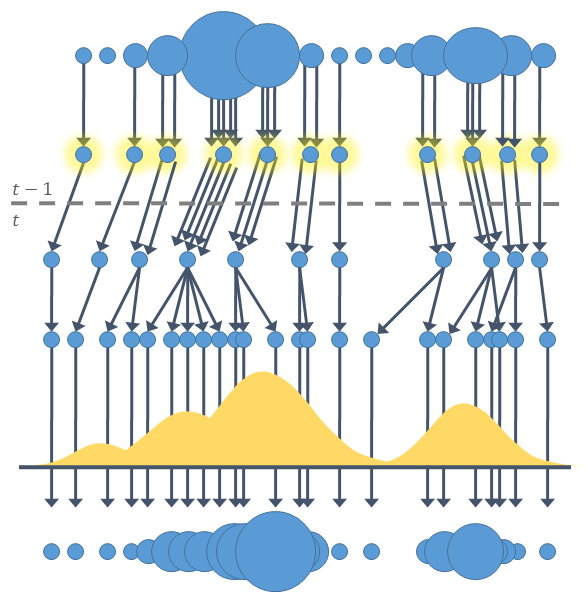
\includegraphics[width=0.6\textwidth]{figures/resampling.png}
    \caption{Illustration of the resampling step in a bootstrap particle filter. The weighted particles in the first row are replaced by particles in the second row with equal weight but similar probability density.\cite{resampling_image}}
    \label{fig:resampling}
\end{figure}
